%%%%%%%%%%%%%%%%%%%%%%%%%%%%%%%%%%%%%%%%%%%%%%%%%%%%%%%%%%%%%%%%%%%%%%%%%%%%%%
\section {Tightening the selections}


%%%%%%%%%%%%%%%%%%%%%%%%%%%%%%%%%%%%%%%%%%%%%%%%%%%%%%%%%%%%%%%%%%%%%%%%%%%%%%
\subsection{Standard selection - distributions of the ID variables }

\begin{figure}[H]
  \begin{tikzpicture}
    \node[anchor=south west,inner sep=0] at (-0.2,0.) {
      % \node[shift={(0 cm,0.cm)},inner sep=0,rotate={90}] at (0,0) {}
      %\makebox[\textwidth][c] {
        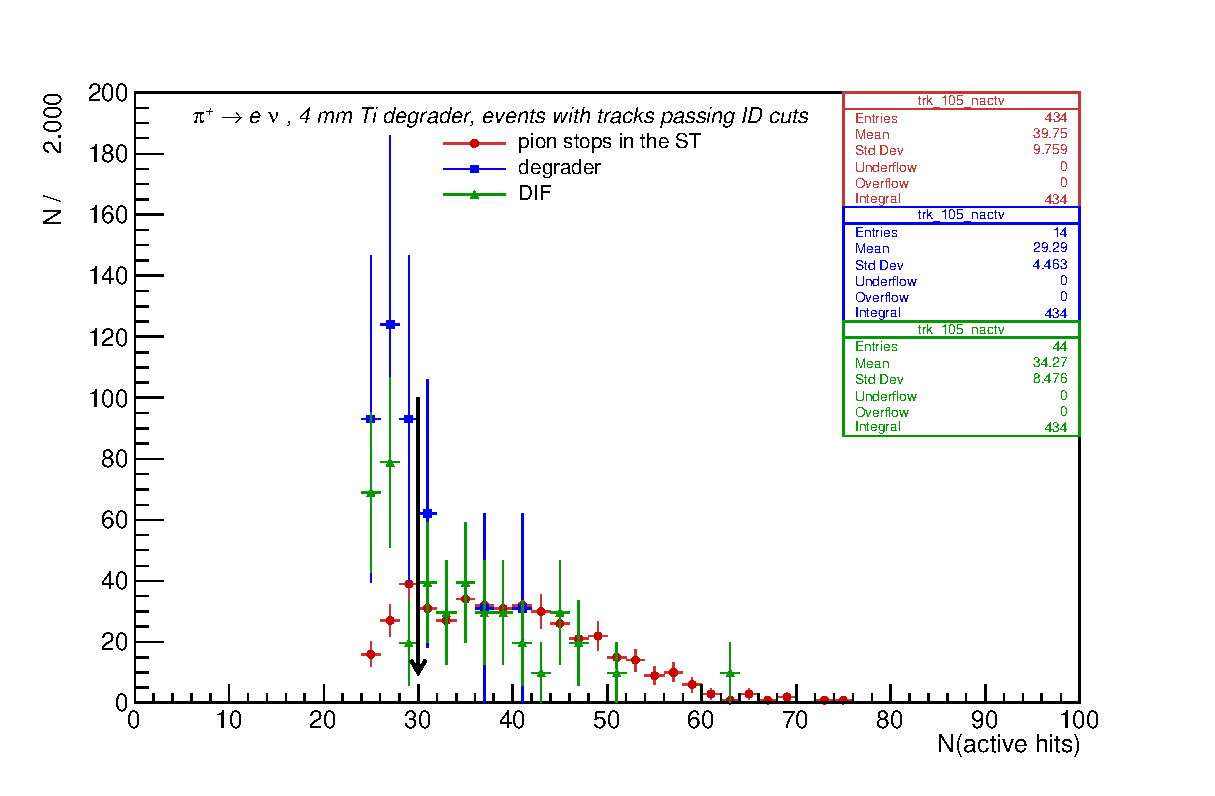
\includegraphics[width=0.58\textwidth]{pdf/figure_00484}
      %}
    };
    \node[anchor=south west,inner sep=0] at (9.7,0.) {
      % \node[shift={(0 cm,0.cm)},inner sep=0,rotate={90}] at (0,0) {}
      % \makebox[\textwidth][c] {
      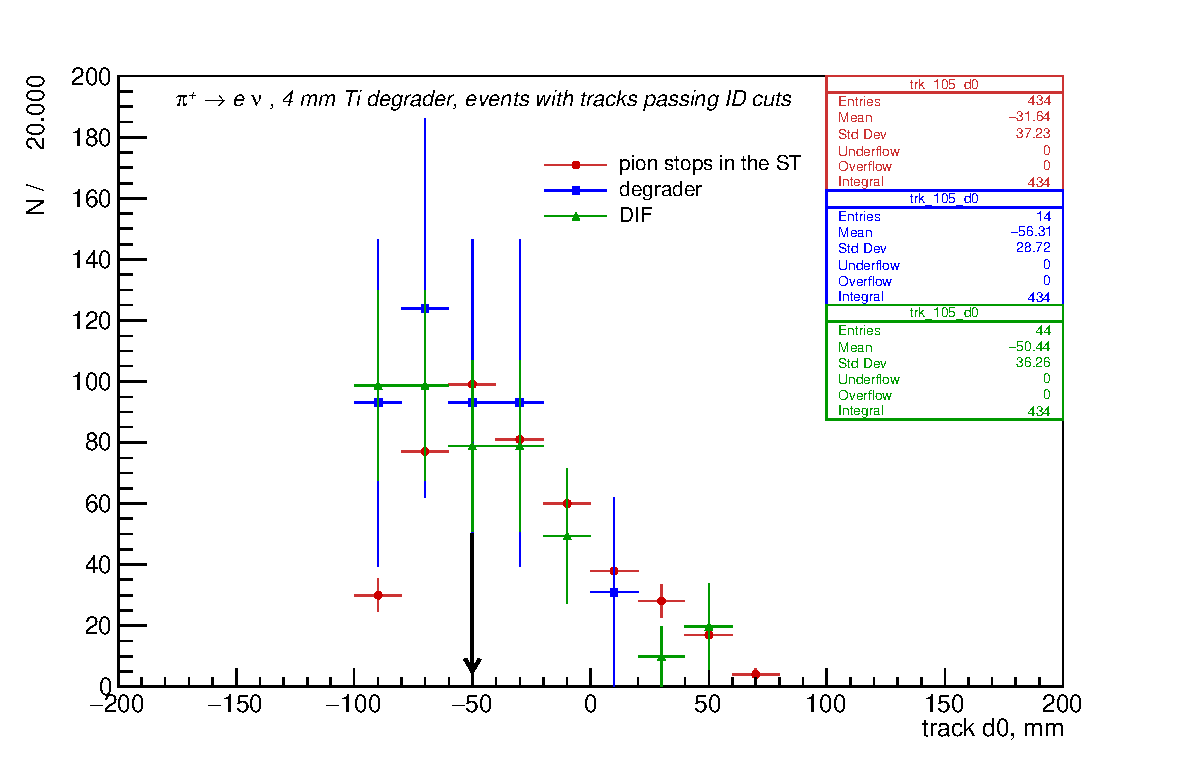
\includegraphics[width=0.58\textwidth]{pdf/figure_00487}
      % }
    };
    % \node [text width=8cm, scale=1.0] at (14.5,0.5) {$\mu_B$, expected background mean};
    % \node [text width=8cm, scale=1.0, rotate={90}] at (1.5,7.5) { $S_{D}$, ``discovery'' signal strength  };
  \end{tikzpicture}
  \caption{
    \label{figure:id_vars_for_events_passed_loose_cits}
    Distributions 
  }
\end{figure}

Figure~\ref{figure:id_vars_for_events_passed_loose_cits} presents distributions for ID variables
for events passing standard ID cuts. The DIF background can be further suppressed with respect to
the signale by tightening the cuts on the number of active hits and the track d0.

Tightening the ID cuts reduces the total DIF background by a significant factor, 10-100.
DIF events with $p < 55$ MeV/c are eliminated, as shown in Figure~\ref{figure:dif_mom_tight_vs_loose}.

Another effect is that the remaining background flattens, and the estimate of the $\pi \to e^+ \nu$
peak position becomes less sensitive to its presence.

\begin{figure}[H]
  \begin{tikzpicture}
    \node[anchor=south west,inner sep=0] at (-0.2,6.5) {
      % \node[shift={(0 cm,0.cm)},inner sep=0,rotate={90}] at (0,0) {}
      % \makebox[\textwidth][c] {
        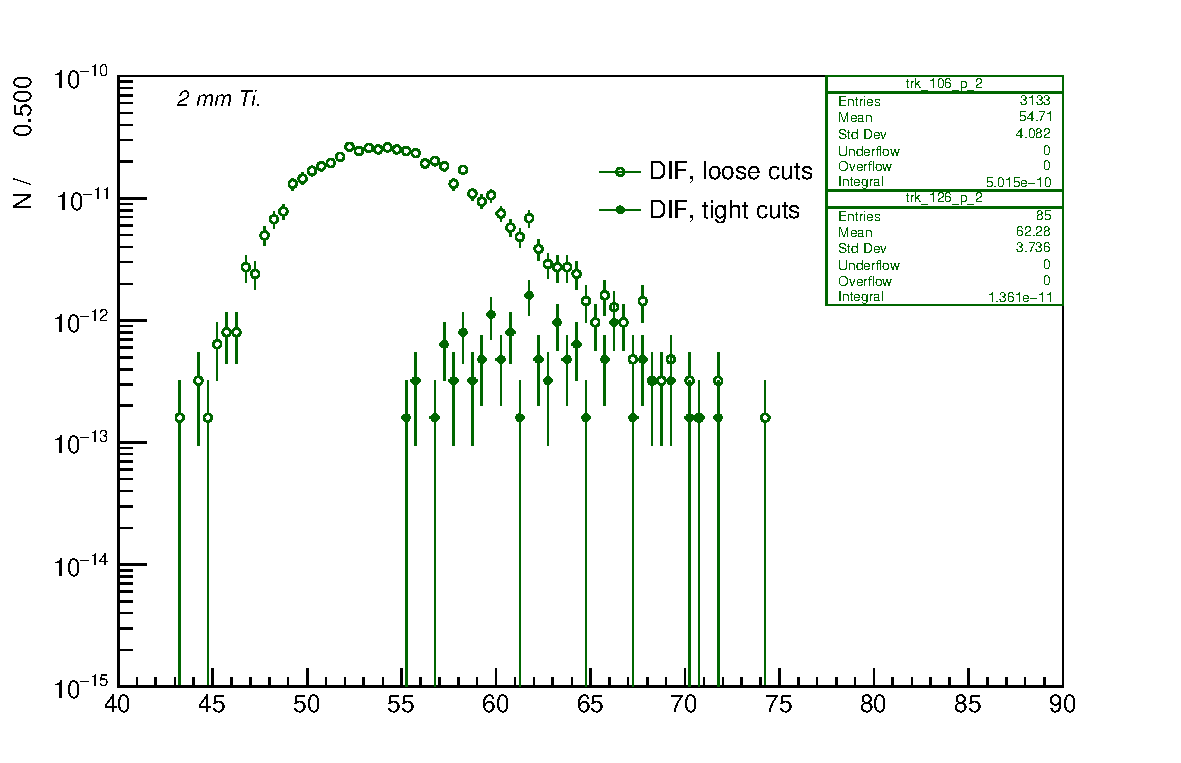
\includegraphics[width=0.58\textwidth]{pdf/figure_00233}
      % }
    };
    \node[anchor=south west,inner sep=0] at (9.5,6.5) {
      % \node[shift={(0 cm,0.cm)},inner sep=0,rotate={90}] at (0,0) {}
      % \makebox[\textwidth][c] {
      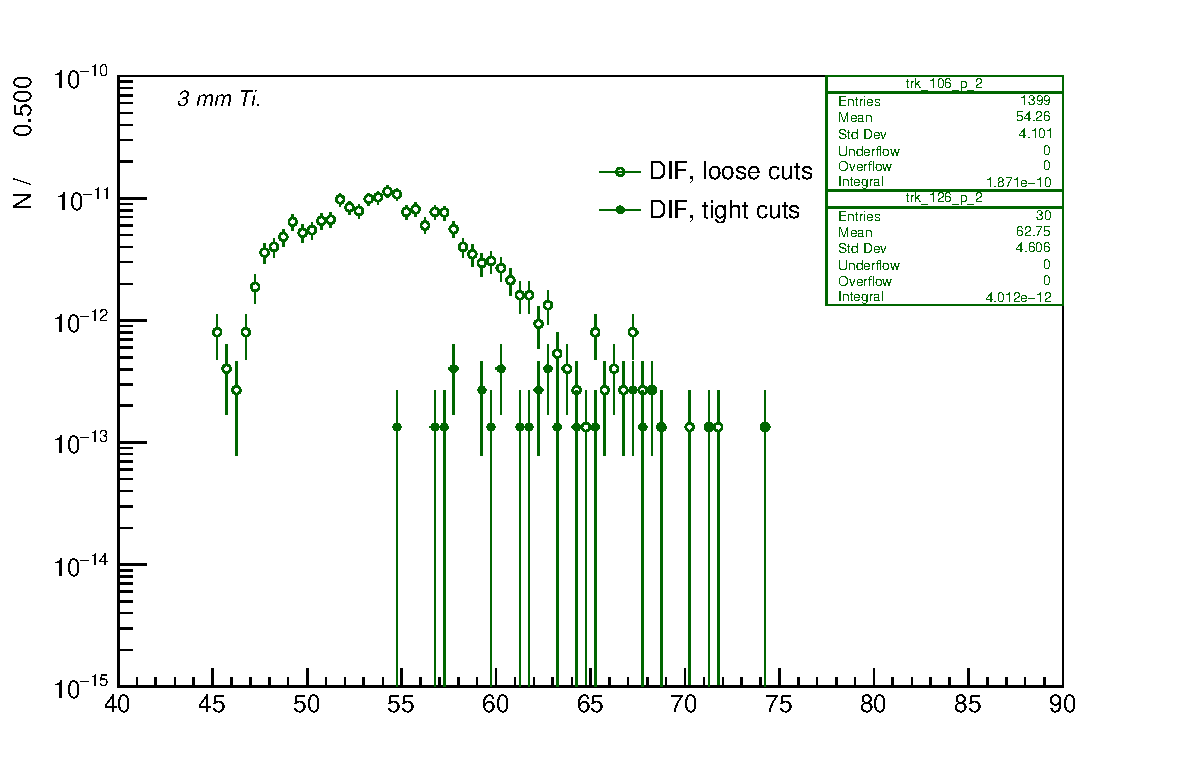
\includegraphics[width=0.58\textwidth]{pdf/figure_00333}
      % }
    };
    \node[anchor=south west,inner sep=0] at (-0.2,0.) {
      % \node[shift={(0 cm,0.cm)},inner sep=0,rotate={90}] at (0,0) {}
      % \makebox[\textwidth][c] {
        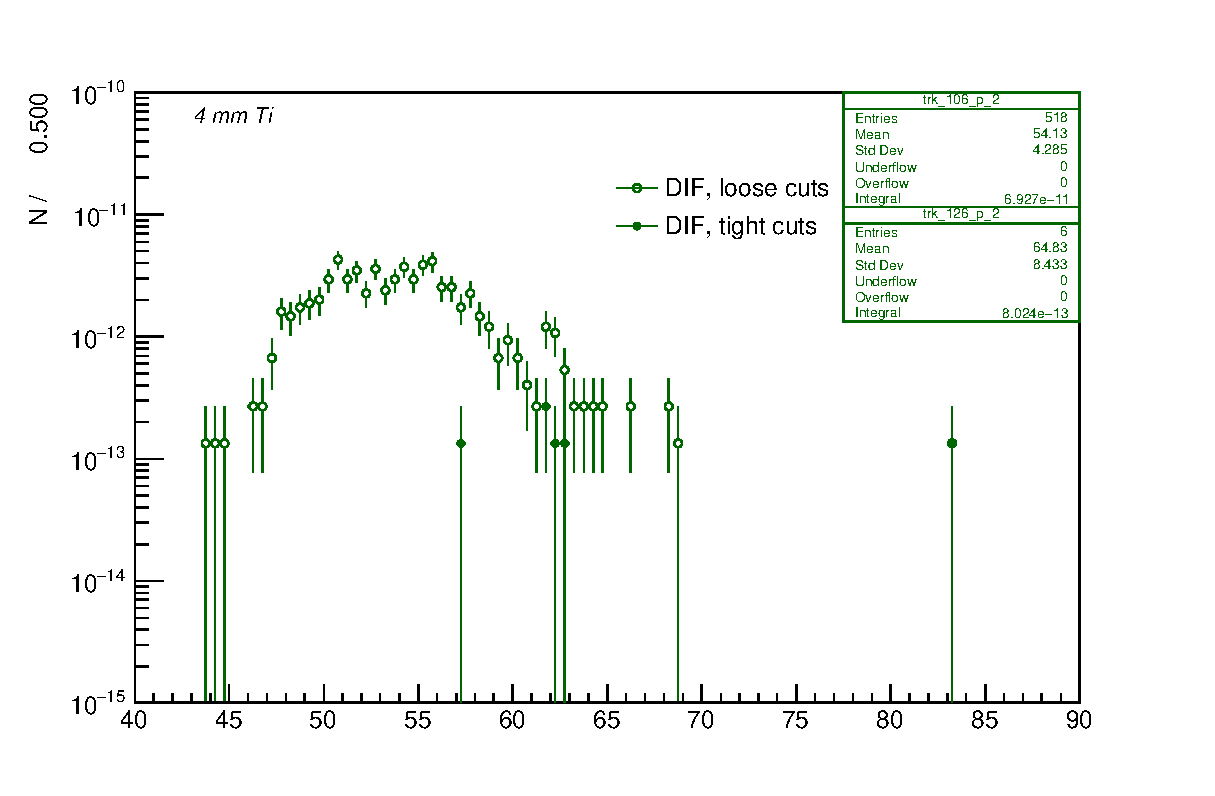
\includegraphics[width=0.58\textwidth]{pdf/figure_00433}
      % }
    };
    \node[anchor=south west,inner sep=0] at (9.5,0.) {
      % \node[shift={(0 cm,0.cm)},inner sep=0,rotate={90}] at (0,0) {}
      % \makebox[\textwidth][c] {
      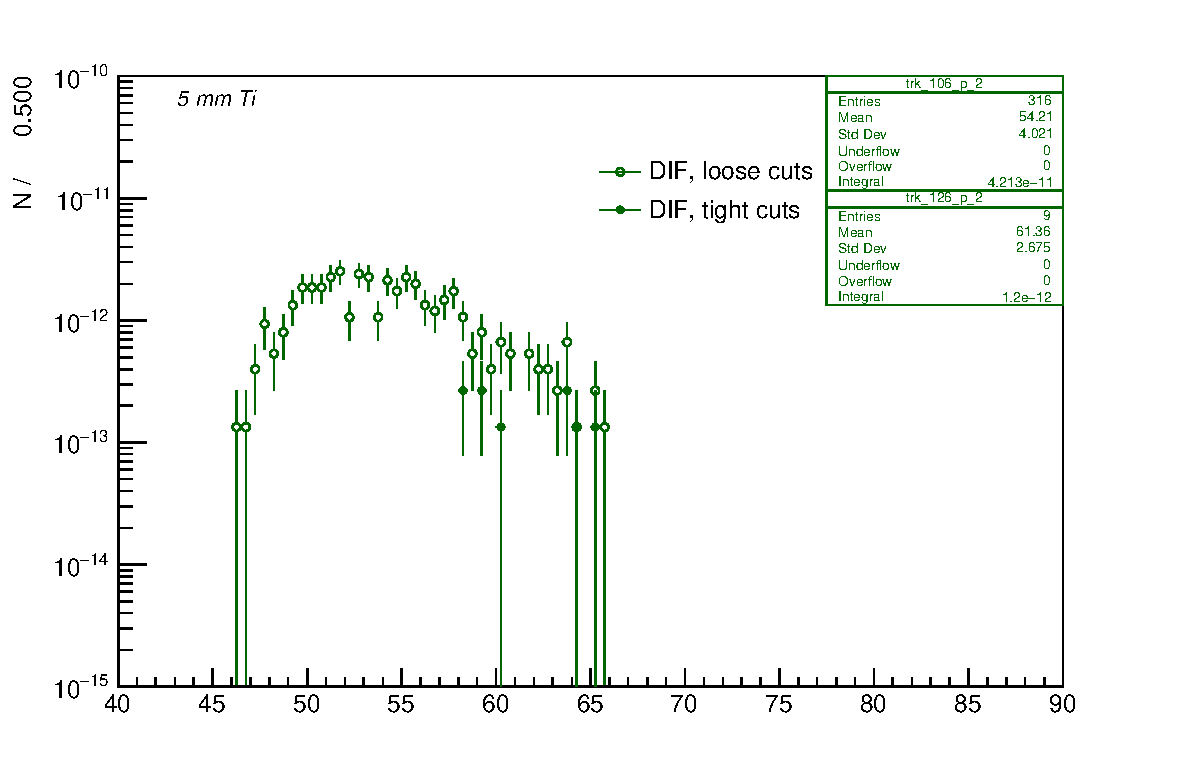
\includegraphics[width=0.58\textwidth]{pdf/figure_00533}
      % }
    };
    % \node [text width=8cm, scale=1.0] at (14.5,0.5) {$\mu_B$, expected background mean};
    % \node [text width=8cm, scale=1.0, rotate={90}] at (1.5,7.5) { $S_{D}$, ``discovery'' signal strength  };
  \end{tikzpicture}
  \caption{
    \label{figure:dif_mom_tight_vs_loose}
    Momentum distributions for DIF ,  tight cuts vs loose cuts.
    Tightening the cuts reduces the DIF background by $\sim$ x50
  }
\end{figure}


Figure~\ref{figure:money_plot_tight_cuts} shows the momentum distributions after
the tight ID cuts are applied.

\begin{figure}[H]
  \begin{tikzpicture}
    \node[anchor=south west,inner sep=0] at (-0.2,6.5) {
      % \node[shift={(0 cm,0.cm)},inner sep=0,rotate={90}] at (0,0) {}
      % \makebox[\textwidth][c] {
        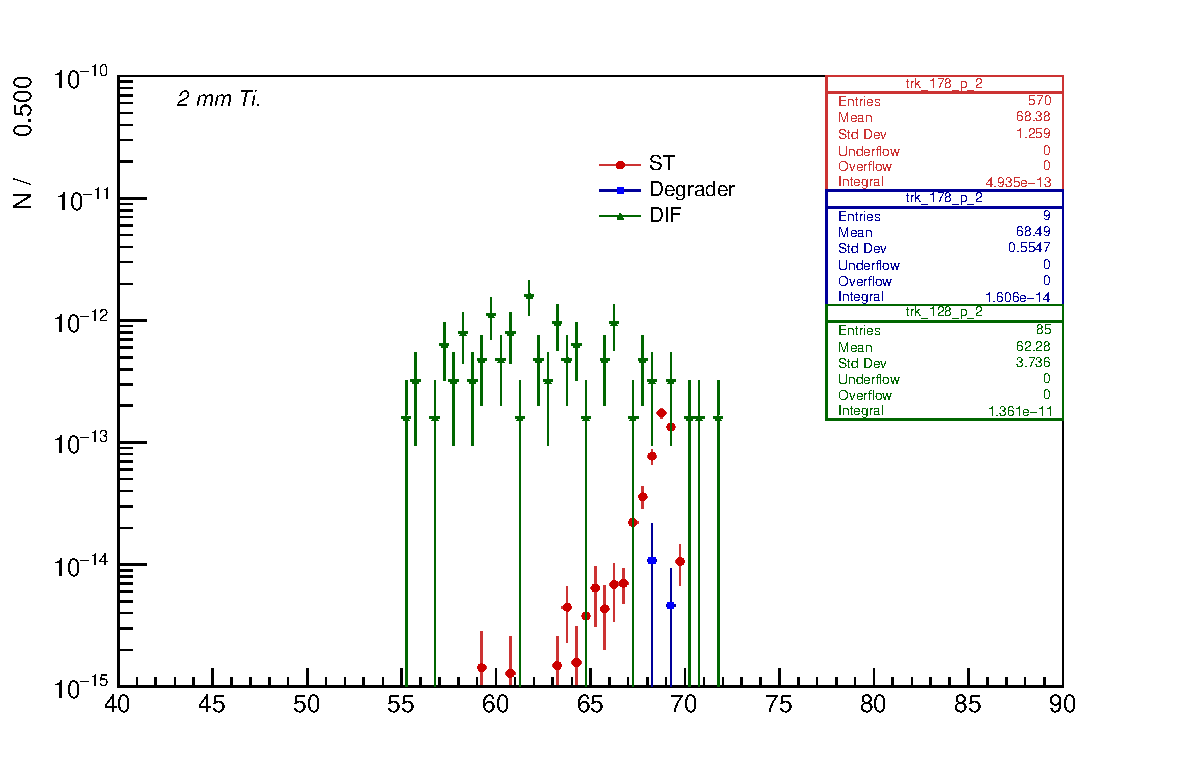
\includegraphics[width=0.58\textwidth]{pdf/figure_00232}
      % }
    };
    \node[anchor=south west,inner sep=0] at (9.5,6.5) {
      % \node[shift={(0 cm,0.cm)},inner sep=0,rotate={90}] at (0,0) {}
      % \makebox[\textwidth][c] {
      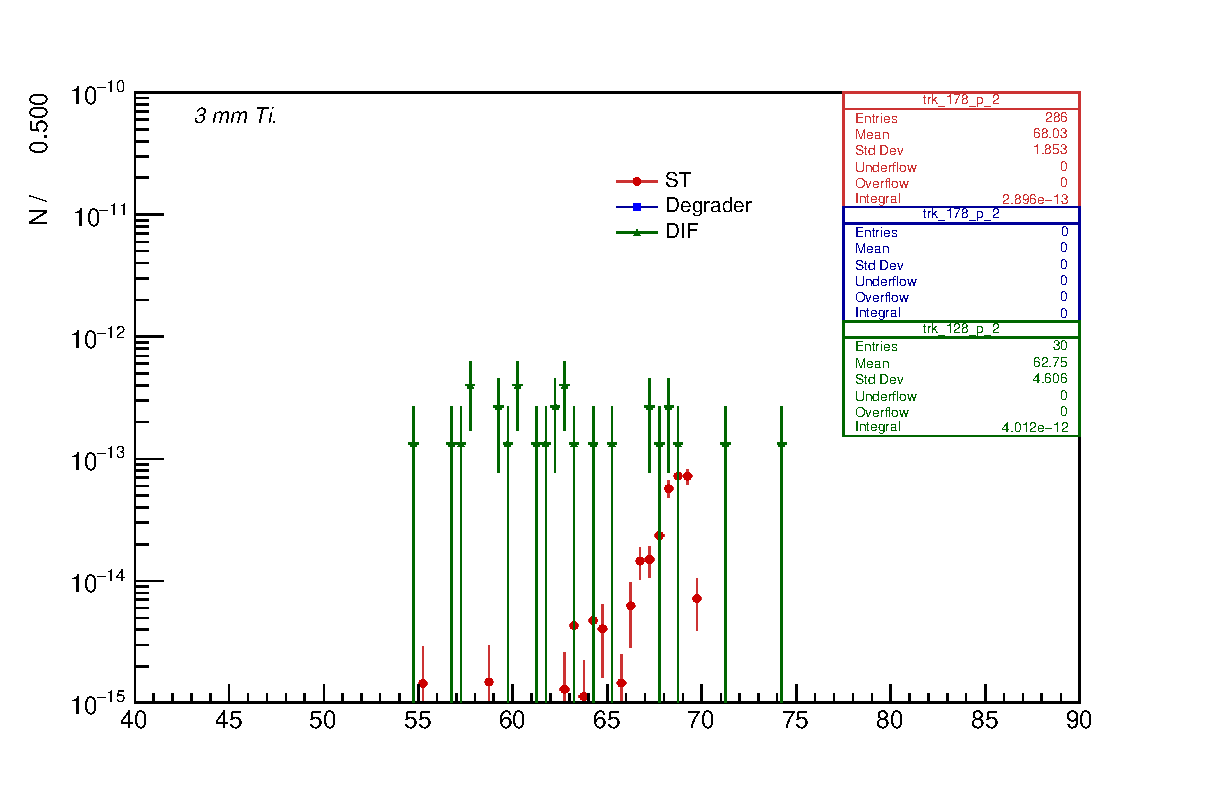
\includegraphics[width=0.58\textwidth]{pdf/figure_00332}
      % }
    };
    \node[anchor=south west,inner sep=0] at (-0.2,0.) {
      % \node[shift={(0 cm,0.cm)},inner sep=0,rotate={90}] at (0,0) {}
      % \makebox[\textwidth][c] {
        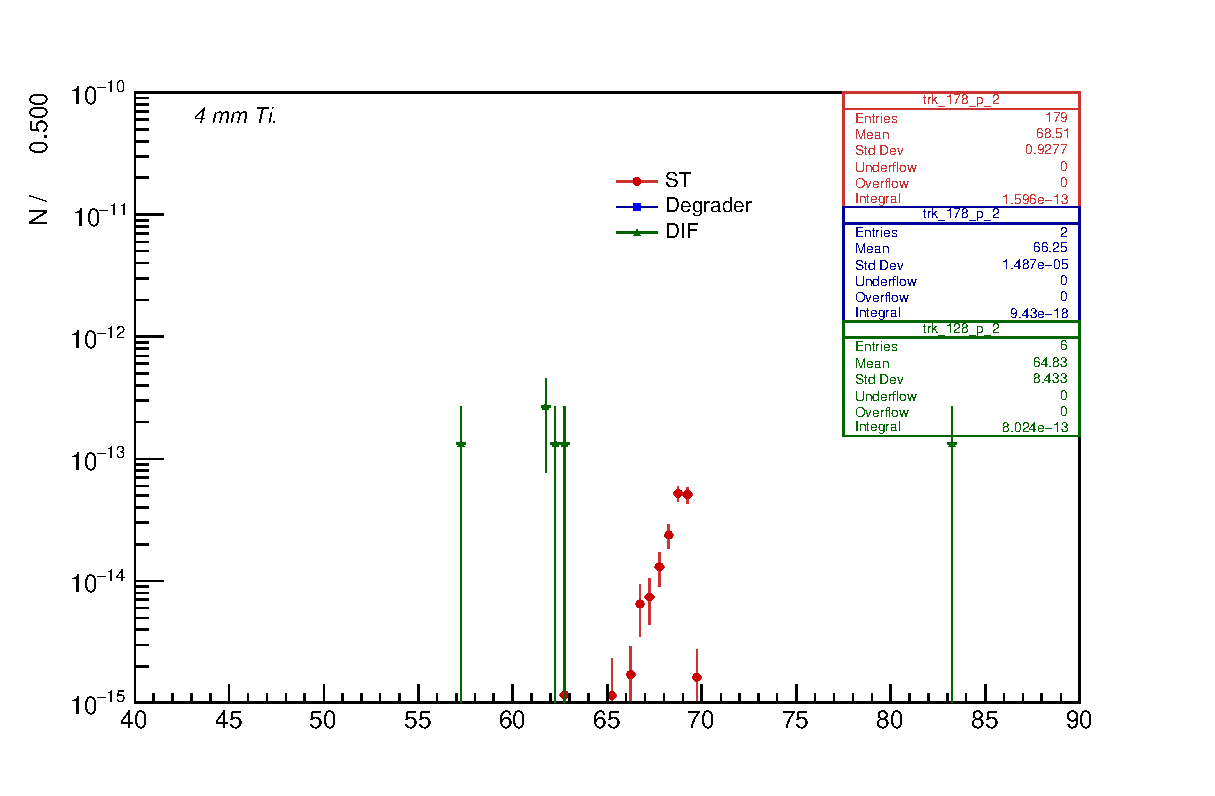
\includegraphics[width=0.58\textwidth]{pdf/figure_00432}
      % }
    };
    \node[anchor=south west,inner sep=0] at (9.5,0.) {
      % \node[shift={(0 cm,0.cm)},inner sep=0,rotate={90}] at (0,0) {}
      % \makebox[\textwidth][c] {
      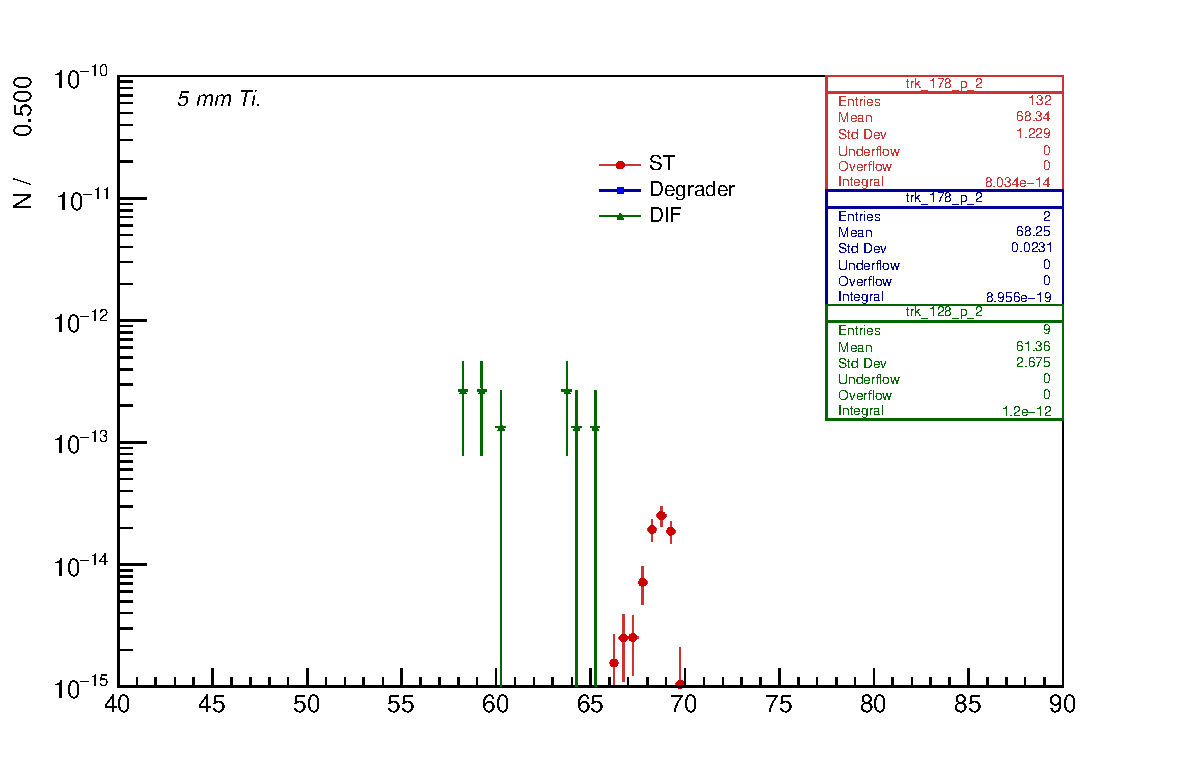
\includegraphics[width=0.58\textwidth]{pdf/figure_00532}
      % }
    };
    % \node [text width=8cm, scale=1.0] at (14.5,0.5) {$\mu_B$, expected background mean};
    % \node [text width=8cm, scale=1.0, rotate={90}] at (1.5,7.5) { $S_{D}$, ``discovery'' signal strength  };
  \end{tikzpicture}
  \caption{
    \label{figure:money_plot_tight_cuts}
    Momentum distributions, tight cuts.
  }
\end{figure}

Present MC statistics doesn't allow to estimate the background under the $\pi^+ \to e^+ \nu$ peak.

There is an indication that a favorable S/B ratio can be achieved for 4 mm and 5mm
Ti degrader thicknesses.

An increase in the MC statistics by at an order of magnitude is required to reach
a meaningful conclusion.

%%% Local Variables:
%%% mode: latex
%%% TeX-master: "mu2e-xxxxx"
%%% End:
